% id: 174-23
% book: 베이직쎈 대수 · 10 등비수열
% section: 유형 106 등비수열의 활용
% figure: tikz:fig-174-23
% answer: 
% answer_source: 
% variant_level: 0 (원본 전사)
% 이 파일은 build.mjs 가 items.json 에서 만든다. 고칠 때는 items.json 을 고친다.
\smash{\raisebox{1.5mm}{\dmkichul{베이직쎈 대수 174쪽 23번}}}
\noindent\begin{minipage}[t]{0.58\linewidth}\vspace{0pt}\raggedright 한 변의 길이가 $3$인 정사각형이 있다. 첫 번째 시행에서 오른쪽 그림과 같이 정사각형을 9등분 하여 중앙의 정사각형을 버린다. 두 번째 시행에서는 첫 번째 시행 후 남은 8개의 정사각형을 각각 9등분 하여 중앙의 정사각형을 버린다. 이와 같은 시행을 계속할 때, 열 번째 시행 후 남아 있는 도형의 넓이는 $\dfrac{2^{a}}{3^{b}}$이다. 이때 자연수 $a$, $b$에 대하여 $a-b$의 값을 구하시오.\end{minipage}\hfill\begin{minipage}[t]{0.4\linewidth}\vspace{0pt}\centering \resizebox{\ifdim\width>\linewidth\linewidth\else\width\fi}{!}{% 174-23(174쪽) — 한 변의 길이가 3인 정사각형을 9등분 해 중앙의 정사각형을 버린 1회 시행 뒤의 모습(색칠한 정사각형 8개).
% 스캔 그림이 흐려 TikZ 로 다시 그렸다. 라벨은 원문에 있는 3 만 두고 남은 넓이(답)는 적지 않는다.
% 격자는 step= 을 쓰면 시작 모서리 선이 빠지므로 \foreach 로 직접 긋는다.
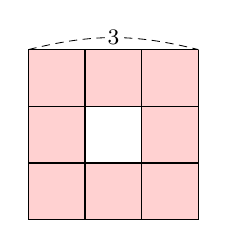
\begin{tikzpicture}[scale=0.72, line width=0.5pt]
  \fill[red!18] (0,0) rectangle (3,3);
  \fill[white] (1,1) rectangle (2,2);
  \foreach \i in {0,1,2,3} {
    \draw (\i,0) -- (\i,3);
    \draw (0,\i) -- (3,\i);
  }
  \draw[densely dashed, line width=0.3pt] (0,3)
    to[bend left=14] node[midway, fill=white, inner sep=1pt, font=\footnotesize] {$3$} (3,3);
\end{tikzpicture}
}\end{minipage}\par
